

\tikzset{every picture/.style={line width=0.75pt}} %set default line width to 0.75pt        

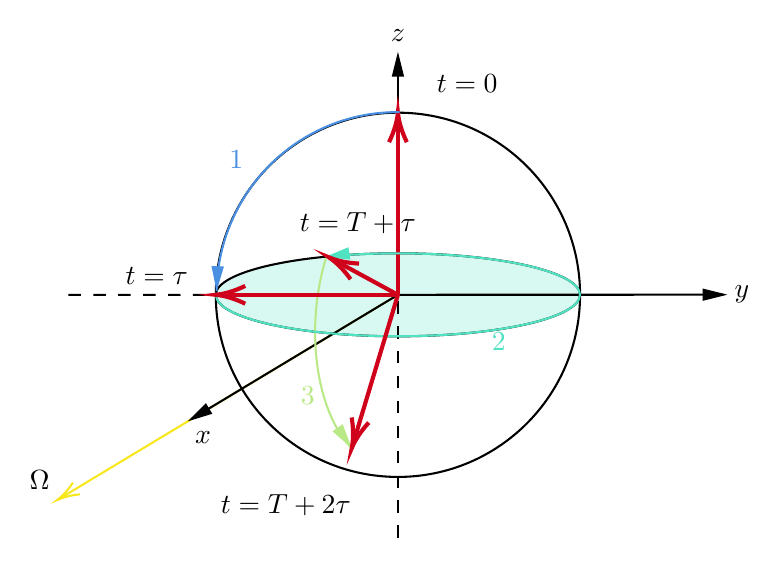
\begin{tikzpicture}[x=0.75pt,y=0.75pt,yscale=-1,xscale=1]
%uncomment if require: \path (0,312); %set diagram left start at 0, and has height of 312

%Straight Lines [id:da7848980629300351] 
\draw [color={rgb, 255:red, 248; green, 231; blue, 28 }  ,draw opacity=1 ]   (200.75,171.75) -- (38.21,269.66) ;
\draw [shift={(36.5,270.69)}, rotate = 328.94] [color={rgb, 255:red, 248; green, 231; blue, 28 }  ,draw opacity=1 ][line width=0.75]    (10.93,-3.29) .. controls (6.95,-1.4) and (3.31,-0.3) .. (0,0) .. controls (3.31,0.3) and (6.95,1.4) .. (10.93,3.29)   ;
%Shape: Circle [id:dp2022100392404811] 
\draw   (113,171.75) .. controls (113,123.29) and (152.29,84) .. (200.75,84) .. controls (249.21,84) and (288.5,123.29) .. (288.5,171.75) .. controls (288.5,220.21) and (249.21,259.5) .. (200.75,259.5) .. controls (152.29,259.5) and (113,220.21) .. (113,171.75) -- cycle ;
%Shape: Ellipse [id:dp11699912573923155] 
\draw  [fill={rgb, 255:red, 80; green, 227; blue, 194 }  ,fill opacity=0.23 ] (113,171.75) .. controls (113,160.7) and (152.29,151.75) .. (200.75,151.75) .. controls (249.21,151.75) and (288.5,160.7) .. (288.5,171.75) .. controls (288.5,182.8) and (249.21,191.75) .. (200.75,191.75) .. controls (152.29,191.75) and (113,182.8) .. (113,171.75) -- cycle ;
%Straight Lines [id:da050591265379689165] 
\draw    (200.75,171.75) -- (200.75,56.69) ;
\draw [shift={(200.75,54.69)}, rotate = 90] [fill={rgb, 255:red, 0; green, 0; blue, 0 }  ][line width=0.08]  [draw opacity=0] (12,-3) -- (0,0) -- (12,3) -- cycle    ;
%Straight Lines [id:da550944948978433] 
\draw    (200.75,171.75) -- (357.5,171.69) ;
\draw [shift={(359.5,171.69)}, rotate = 179.98] [fill={rgb, 255:red, 0; green, 0; blue, 0 }  ][line width=0.08]  [draw opacity=0] (12,-3) -- (0,0) -- (12,3) -- cycle    ;
%Straight Lines [id:da7132616118498538] 
\draw    (200.75,171.75) -- (101.21,231.66) ;
\draw [shift={(99.5,232.69)}, rotate = 328.96] [fill={rgb, 255:red, 0; green, 0; blue, 0 }  ][line width=0.08]  [draw opacity=0] (12,-3) -- (0,0) -- (12,3) -- cycle    ;
%Straight Lines [id:da19326397751399682] 
\draw  [dash pattern={on 4.5pt off 4.5pt}]  (42,171.81) -- (200.75,171.75) ;
%Straight Lines [id:da5007447778090508] 
\draw [color={rgb, 255:red, 208; green, 2; blue, 27 }  ,draw opacity=1 ][line width=1.5]    (200.75,171.75) -- (200.75,87) ;
\draw [shift={(200.75,84)}, rotate = 90] [color={rgb, 255:red, 208; green, 2; blue, 27 }  ,draw opacity=1 ][line width=1.5]    (14.21,-4.28) .. controls (9.04,-1.82) and (4.3,-0.39) .. (0,0) .. controls (4.3,0.39) and (9.04,1.82) .. (14.21,4.28)   ;
%Straight Lines [id:da8090900757565247] 
\draw [color={rgb, 255:red, 74; green, 144; blue, 226 }  ,draw opacity=1 ]   (113.71,162.69) -- (113.47,167.98) ;
\draw [shift={(113.39,169.98)}, rotate = 272.53] [fill={rgb, 255:red, 74; green, 144; blue, 226 }  ,fill opacity=1 ][line width=0.08]  [draw opacity=0] (12,-3) -- (0,0) -- (12,3) -- cycle    ;
%Straight Lines [id:da59853592736301] 
\draw [color={rgb, 255:red, 80; green, 227; blue, 194 }  ,draw opacity=1 ]   (168.31,153.14) -- (167.47,153.26) ;
\draw [shift={(165.5,153.55)}, rotate = 351.68] [fill={rgb, 255:red, 80; green, 227; blue, 194 }  ,fill opacity=1 ][line width=0.08]  [draw opacity=0] (12,-3) -- (0,0) -- (12,3) -- cycle    ;
%Straight Lines [id:da8934478617364343] 
\draw  [dash pattern={on 4.5pt off 4.5pt}]  (200.75,288.81) -- (200.75,171.75) ;
%Shape: Arc [id:dp3798664572181705] 
\draw  [draw opacity=0] (178.5,245.69) .. controls (172.04,239.07) and (166.78,228.83) .. (163.69,215.56) .. controls (159.05,195.64) and (160.3,173.18) .. (166.02,154.23) -- (200.82,183.24) -- cycle ; \draw  [color={rgb, 255:red, 184; green, 233; blue, 134 }  ,draw opacity=1 ] (178.5,245.69) .. controls (172.04,239.07) and (166.78,228.83) .. (163.69,215.56) .. controls (159.05,195.64) and (160.3,173.18) .. (166.02,154.23) ;
%Shape: Arc [id:dp27150518666038126] 
\draw  [draw opacity=0] (113.39,169.98) .. controls (114.14,122.23) and (152.8,83.75) .. (200.38,83.75) .. controls (200.78,83.75) and (201.18,83.75) .. (201.58,83.76) -- (200.38,171.41) -- cycle ; \draw  [color={rgb, 255:red, 74; green, 144; blue, 226 }  ,draw opacity=1 ] (113.39,169.98) .. controls (114.14,122.23) and (152.8,83.75) .. (200.38,83.75) .. controls (200.78,83.75) and (201.18,83.75) .. (201.58,83.76) ;
%Shape: Arc [id:dp5432770976020507] 
\draw  [draw opacity=0] (168.45,153.16) .. controls (178.45,152.26) and (189.35,151.77) .. (200.75,151.77) .. controls (249.19,151.77) and (288.46,160.71) .. (288.46,171.75) .. controls (288.46,182.79) and (249.19,191.73) .. (200.75,191.73) .. controls (152.31,191.73) and (113.04,182.79) .. (113.04,171.75) .. controls (113.04,171.42) and (113.08,171.1) .. (113.14,170.77) -- (200.75,171.75) -- cycle ; \draw  [color={rgb, 255:red, 80; green, 227; blue, 194 }  ,draw opacity=1 ] (168.45,153.16) .. controls (178.45,152.26) and (189.35,151.77) .. (200.75,151.77) .. controls (249.19,151.77) and (288.46,160.71) .. (288.46,171.75) .. controls (288.46,182.79) and (249.19,191.73) .. (200.75,191.73) .. controls (152.31,191.73) and (113.04,182.79) .. (113.04,171.75) .. controls (113.04,171.42) and (113.08,171.1) .. (113.14,170.77) ;
%Straight Lines [id:da9377445119383205] 
\draw [color={rgb, 255:red, 208; green, 2; blue, 27 }  ,draw opacity=1 ][line width=1.5]    (200.75,171.75) -- (116,171.75) ;
\draw [shift={(113,171.75)}, rotate = 360] [color={rgb, 255:red, 208; green, 2; blue, 27 }  ,draw opacity=1 ][line width=1.5]    (14.21,-4.28) .. controls (9.04,-1.82) and (4.3,-0.39) .. (0,0) .. controls (4.3,0.39) and (9.04,1.82) .. (14.21,4.28)   ;
%Straight Lines [id:da34551979860290394] 
\draw [color={rgb, 255:red, 208; green, 2; blue, 27 }  ,draw opacity=1 ][line width=1.5]    (200.75,171.75) -- (170.14,155.12) ;
\draw [shift={(167.5,153.69)}, rotate = 28.51] [color={rgb, 255:red, 208; green, 2; blue, 27 }  ,draw opacity=1 ][line width=1.5]    (14.21,-4.28) .. controls (9.04,-1.82) and (4.3,-0.39) .. (0,0) .. controls (4.3,0.39) and (9.04,1.82) .. (14.21,4.28)   ;
%Straight Lines [id:da9440630200952458] 
\draw [color={rgb, 255:red, 184; green, 233; blue, 134 }  ,draw opacity=1 ]   (176.8,243.22) -- (177.37,244.04) ;
\draw [shift={(178.5,245.69)}, rotate = 235.43] [fill={rgb, 255:red, 184; green, 233; blue, 134 }  ,fill opacity=1 ][line width=0.08]  [draw opacity=0] (12,-3) -- (0,0) -- (12,3) -- cycle    ;
%Straight Lines [id:da6204836007465544] 
\draw [color={rgb, 255:red, 208; green, 2; blue, 27 }  ,draw opacity=1 ][line width=1.5]    (200.75,171.75) -- (179.36,242.81) ;
\draw [shift={(178.5,245.69)}, rotate = 286.75] [color={rgb, 255:red, 208; green, 2; blue, 27 }  ,draw opacity=1 ][line width=1.5]    (14.21,-4.28) .. controls (9.04,-1.82) and (4.3,-0.39) .. (0,0) .. controls (4.3,0.39) and (9.04,1.82) .. (14.21,4.28)   ;

% Text Node
\draw (200.75,51.29) node [anchor=south] [inner sep=0.75pt]    {$z$};
% Text Node
\draw (101.5,236.09) node [anchor=north west][inner sep=0.75pt]    {$x$};
% Text Node
\draw (361.5,171.69) node [anchor=west] [inner sep=0.75pt]    {$y$};
% Text Node
\draw (34.5,267.29) node [anchor=south east] [inner sep=0.75pt]    {$\boldsymbol{\Omega }$};
% Text Node
\draw (218,64.4) node [anchor=north west][inner sep=0.75pt]    {$t=0$};
% Text Node
\draw (101,168.35) node [anchor=south east] [inner sep=0.75pt]    {$t=\tau $};
% Text Node
\draw (152,130.4) node [anchor=north west][inner sep=0.75pt]    {$t=T+\tau $};
% Text Node
\draw (118,101) node [anchor=north west][inner sep=0.75pt]  [color={rgb, 255:red, 74; green, 144; blue, 226 }  ,opacity=1 ] [align=left] {1};
% Text Node
\draw (244.5,188.5) node [anchor=north west][inner sep=0.75pt]  [color={rgb, 255:red, 80; green, 227; blue, 194 }  ,opacity=1 ] [align=left] {2};
% Text Node
\draw (114,266.4) node [anchor=north west][inner sep=0.75pt]    {$t=T+2\tau $};
% Text Node
\draw (152.5,214.5) node [anchor=north west][inner sep=0.75pt]  [color={rgb, 255:red, 184; green, 233; blue, 134 }  ,opacity=1 ] [align=left] {3};


\end{tikzpicture}
